\section{Discussion}

Note: similarly no impact on rental market (as rents are always at max capacity). The ogernment should focus on insulation. we also need to distinguish between all homes and rental properties when mentioning the figures below. Are the cost tables 3, 4 and 5 for all properties or just rentals? (we will need both).


Imposing a stricter energy efficiency standard (MEES) of 69 on all dwellings capable of reaching such standards has the potential of decreasing the UK's housing annual emissions by 38.2-42.5\% from 2022 levels \footnote{values determined from EPC retrofitting strategy for both houses able and unable to reach 69.} (and 52.3 - 55.6\% from 2017 baseline levels) \cite{department_for_business_energy_and_industrial_strategy_english_2023, department_for_business_energy_and_industrial_strategy_household_2020, office_for_national_statistics_energy_2023}.  If $8.2$ million properties retrofit to an EPC of C within 2028 - as recommended by the CCC \cite{climate_change_committee_ccc_2022_2022} - the UK housing sector would surpass its NZ targets of decreasing 50\%  of  residential emissions by 2032 compared to 2017 \cite{department_for_business_energy_and_industrial_strategy_english_2023}. The UK could be well on the road to Net Zero. While setting MEES could serve as a critical pathway for England and Wales to meet their Net Zero goals by 2050, the success of the policy amendment must be weighed against the financial incentives for households and the broader impacts on the already challenging domestic housing sector. \\

Households across England and Wales would have to bear a cost of \textsterling $91.6$ billion \footnote{This figure includes \textsterling 82.5 to reach an EPC of C and \textsterling9.1 for all other dwellings to reach their maximum energy efficiency potential.} in energy improvements  to reach a minimum EPC standard of C (score of 69 out of 100) - or at least maximum efficiency potential with the current ceiling. Results indicate over \textsterling 29 billion would be spent on wall insulation (ID 7), followed by \textsterling 13 billion in solar water heating technologies (ID 19). The overall costs of these two technologies have not significantly come down in recent years, sitting at \textsterling10,000-9,000 and \textsterling 5,000 - respectively. These were possibly induced by a lack of demand and 'experience learning-curve' effect \cite{lafond_how_2018, zhou_learning_2019, bosetti_witch_2006} as uptake of solar water heaters and wall insulation measures had remained low in the past - despite government incentives and EPC recommendations \cite{hamilton_uptake_2014}. The average retrofitting cost at household level of 
reaching MEES ranges from \textsterling 6,434 to \textsterling 10,000 based on three different retrofitting strategies. However, as with aggregate costs, such prices may be overestimated as experiential learning curves and economies of scale have not been taken into consideration \cite{lafond_how_2018}. Should households commit to retrofits as suggested in their EPC reports, the resulted cost would be higher than identifying the most impactful retrofits with respect to price per price. 

This is concerning as property owners have limited information when deciding to commit to green retrofits and other geographical and time dependent factors are likely to influence this decision as well, including the potential rent premium for higher efficient properties or the surcharge paid for a property due to lack of supply, thus exacerbating inequalities. Landlords might simply decide to sell their rental properties as future rents would not be able to compensate for the upfront costs associated with meeting the new EPC and the loss of rents while retrofits are being conducted. \\


The average retrofitting costs of achieving minimum energy efficiency of 69\% - or highest energy efficiency potential for less-able properties -  vary widely by construction age and price range. Older properties, especially pre-war homes, would have to incur higher retrofitting costs due to their low efficiency. These account for over 35\% of properties in the UK and Wales, with wales having more very old homes \cite{building_research_establishment_housing_2018}. Property owners would have to spend  \textsterling 9-15k in renovations for those able to reach 69\% and \textsterling 8-10k for others to reach their maximum energy efficiency. \\

\begin{figure}[ht]
    \centering
    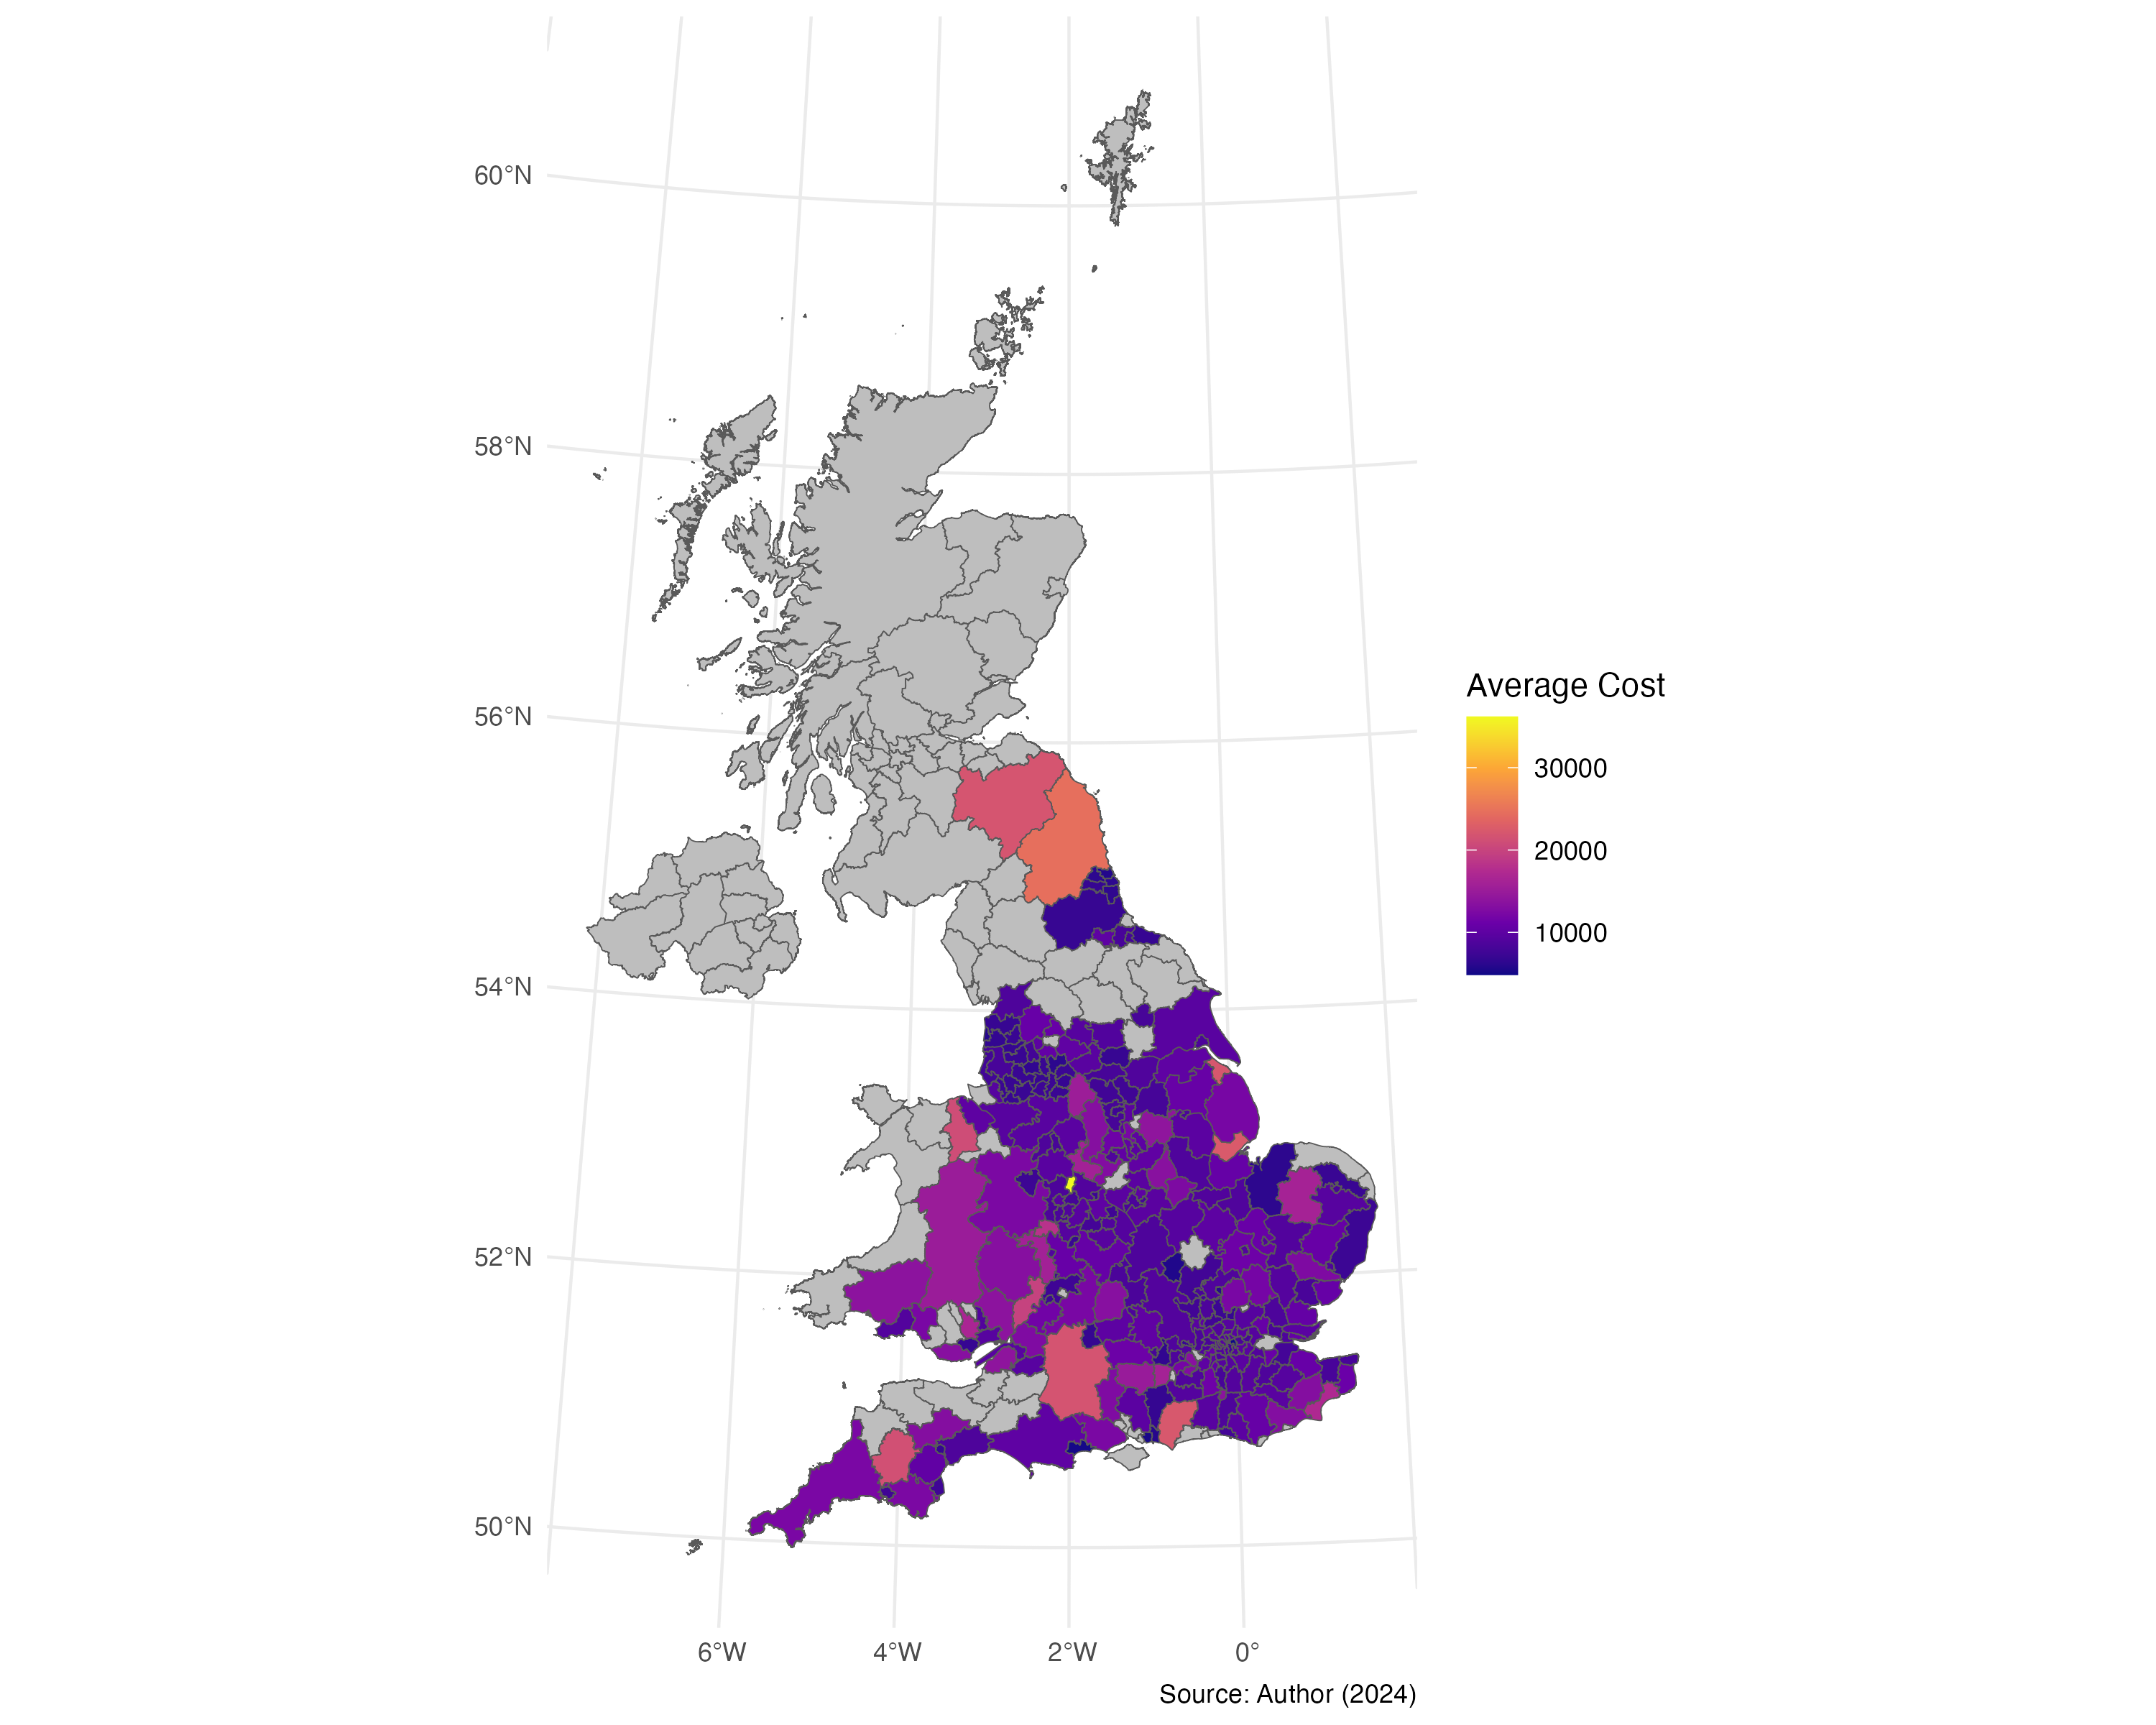
\includegraphics[width=1\linewidth]{src/figures/average_costs_per_district.png}
    \caption{Average retrofitting costs per district in England and Wales (sourced shapesfiles from ONS)}
    \label{fig:costs_district}
\end{figure}

Although not highly geographically heterogeneous (Figure \ref{fig:costs_district}), certain districts seem to show above-average retrofitting costs to reach the new requirements. These correspond to the local authority districts of the Scottish Borders, Northumberland in the Northeast as well as Wiltshire and West Devon in SouthWest which are largely rural  \cite{vera-toscano_ruralurban_2024}. These align with existing reports of unusually high poverty in these districts \cite{baker_profile_2003, scottish_borders_council_lhs_2016}. Fuel poverty is often associated with low income and less-energy efficient households as affordability for energy costs are low \cite{baker_predicting_2003}.


Although the figures therein represent the estimated costs as houses implement recommendations from the EPCs, there is no legal requirement for property owners to follow such order. Instead, a minimum energy efficiency standard - as suggested by the UK government in 2021 - would take a 'whole house retrofit' approach and not take into account the nuances of property-level decisions. However, as seen by the nuances and sensitivity of the costs by retrofitting strategy (\ref{EPC_69_costs}), an surgical approach to retrofitting would capture much more nuances to overall retrofitting costs and total abated emissions \cite{alabid_review_2022, uk_green_building_council_ukgbc_retrofit_2021}.\textbf{ }Indeed, the results confirmed previous studies' criticism on the energy-cost focused narrative of the SAP and RdSAP recommendations \cite{kelly_building_2012} . A more sequential and tailored approach to implementing energy efficiency improvements, prioritizing those with the highest yield, could significantly reduce household costs and facilitate more coordinated investments in specific improvement industries, potentially driving down retrofitting expenses \cite{alabid_review_2022}. As previously discussed, the EPC retrofitting scheme designed to meet the Minimum Energy Efficiency Standards (MEES) has emphasized investments in technologies that are individually expensive and have not demonstrated significant price reductions over time. In contrast, if households were to prioritize improvements that offer the greatest efficiency gains relative to their cost, the majority of aggregate spending would likely be directed towards the installation of solar photovoltaic (PV) panels (ID 34). Such large-scale investment—potentially exceeding £16 billion—could, over time, further reduce retrofitting costs for homeowners as the increasing adoption of PV technology drives economies of scale and fosters technological advancements \cite{lafond_how_2018}. Effective policies in the past have proven to possible to positively affect industry prices and end-user implementation of green innovations.  Indeed, uptake of biogas in countries like India and China have increased as a result of up-to-date policy initiatives \cite{abanades_critical_2022}. Therefore, an effective and demographically tailored regulation on retrofitting schemes would significantly decrease household renovation prices for households while also enabling focused investments green technologies. Further decreasing prices and enabling more properties to reach higher energy efficiencies by reducing financial limits to MEES and making EPC C potentially more affordable under an elemental approach. \\

Only 29\% of retrofitting costs would fall below current energy retrofitting household spending of \textsterling 3,500 as currently implemented by the Private Renting Energy Efficiency Regulations  \cite{department_for_energy_security_and_net_zero_and_department_for_business_energy__industrial_strategy_standard_2023}. Hence, as suggested by the 2021 amendment proposal \cite{department_for_energy_security_and_net_zero_desnz_and_department_for_business_energy_and_industrial_strategy_beis_heat_2021}, an increase in household spending budget would be required to require the desired number of properties to reach an EPC of C. policy makers should consider tailoring this threshold  by property type and construction age. According to the aggregated results therein, the marginal abatement costs for residential emissions can be derived and is estimated at \textsterling 3,273 to \textsterling5,124 per tonne of $CO_2$. This is significant compared to system-wide abatement costs estimated from changing fuel-source of the UK electricity grid \cite{mckinsey_company_appendix_2002}. Suggesting placing all retrofitting costs on end-users to be less efficient than a universal carbon tax to decarbonize the grid and highlighting the importance of introducing system-wide policies in parallel to increasing MEES. 


Several limitation underpin the findings and recommendations suggested above. First, EPCs have been proven as better estimators of energy cost-efficiency \cite{kelly_building_2012}and tend to overestimate energy use \cite{few_over-prediction_2023}. Therefore, more accurate indicators of energy use such as meter data would be preferable to assess post-retrofitting reductions in energy usage. Second, certain types of retrofits are more intrusive than others and require longer installation times resulting in higher costs, further disinventing landlords to commit to these in fear of loss of rental income. Third, the green premium was estimated using a hedonic price model which suffers from different confounding factors, such as demand and supply forces surrounding the point of sale which could result in overestimating the green premium associated with green retrofits. This however provides a ceiling for the estimates in this study. Last, green retrofits might be less costly when committed together as installation costs were computed assuming independent deployment. Improvements, such as cavity wall installations, have also shown not to have long-lasting effects on energy efficiency \cite{penasco_assessing_2023}. By not taking into account such time-varying effects the estimated gains from future energy savings might be overestimated. \\

Future research may want to look further into each aspect of the effects induced by imposed MEES. These may include looking at the specific improvements undertaking by household characteristics and demography to better understand the national-scale investments needed to deploy effective retrofitting strategies. Additionally, while this study could not rely on tenure statistics for more granular estimates, a deeper understanding of the underlying decisions to resale may provide further insights into the market shock produced by imposed standards. Limitations of time and processing power prevented this study from other more robust methods of isolating the effects of certain energy improvements. A potential avenue for investigating such trends would have been to use propensity-score matching (PSM) across properties of similar attributes \cite{fuerst_does_2015, fuerst_energy_2016, penasco_assessing_2023, zhang_price_2017, zhang_does_2021}. \\

To be honest I feel that computing a cost of abatement reveals troubling figures, i.e. the cost per ton of carbon avoided is super high... one conclusion would be that it is much cheaper to decarbonise the grid instead, even if the price of electricity increases drastically it nowhere in the region of what a household would pay. this in itself would be incentive enough to focus on the deployment of renewables. boiler upgrade scheme is 7.5k for gov so how many tons avoided from this once you add up consumer costs? (I can give an asnwer from MCS data BTW)






